\documentclass[12pt]{article}
\usepackage{amssymb}
\usepackage{amsfonts}
\usepackage{amsmath}
\usepackage{amsthm}
\usepackage{titlesec}
\usepackage{fontspec}
\usepackage{lmodern}
\usepackage{dsfont}
\usepackage{color}
\usepackage{fancybox}
\usepackage[margin=0.7in]{geometry}
\usepackage{url}
\usepackage{setspace}
\usepackage{graphicx}
\usepackage{comment}
\usepackage{enumitem}
\usepackage{natbib}
\usepackage{multirow}
\usepackage{indentfirst}
\usepackage{secdot}
\usepackage{siunitx}
\usepackage[bottom]{footmisc}
\usepackage{fancyhdr}
\usepackage{bm}
\usepackage[labelfont=bf, justification=Justified]{caption}
\usepackage[all]{nowidow}
\usepackage{siunitx}
\usepackage{floatrow}
\floatsetup[table]{capposition=top}
\usepackage{booktabs}
\usepackage{afterpage}
\usepackage{longtable}


% set the main font (fontspec package)
\setmainfont{Times New Roman}
%\setmainfont[Renderer=Basic]{Times New Roman}

% change the (sub)section default format
\titleformat{\section}{\normalfont\Large\bfseries}{}{0pt}{}
\titleformat{\subsection}{\normalfont\large\bfseries}{}{0pt}{}
%%\titleformat{\subsubsection}{}{\thesubsubsection)}{1em}{}
%\titleformat{\section}{\normalfont\huge\bfseries}{\thesection}{1em}{}
%\titleformat{\subsection}{\normalfont\large\bfseries\slshape}{\thesubsection)}{1em}{}
%\titleformat{\subsubsection}{\normalfont\normalsize\bfseries\slshape}{\thesubsubsection)}{1em}{}
%
%% change the section numbering to roman literals and subsection to letters and numbers
%\renewcommand{\thesection}{\arabic{section}}
%\renewcommand{\thesubsection}{\alph{subsection}}
%\renewcommand{\thesubsubsection}{\alph{subsection}.\arabic{subsubsection}}

% fonts for source code and files
\renewcommand{\tt}[1]{\textbf{\texttt{#1}}}

% longtable options to force textwidth span
\setlength\LTleft{0pt}
\setlength\LTright{0pt}

% allow page breaking for multiple-line equations
\allowdisplaybreaks


\begin{document}

\title{Machine Learning Methods For Thin Time-Series Data}
\author{Georgios Magkotsios}
\maketitle
\thispagestyle{empty}


\onehalfspacing



\section{Raw data pre-processing}


The column headers in the input spreadsheet are simple numbers. I rename the dependent variable (column ``0'') to $y$ and add a prefix for the rest of the features with the following conventions:
\begin{itemize}
	\item Prefix with $x$ the numerical (continuous) features.
	\item Prefix with $d$ the categorical features. These are already encoded in $[0,1]$ format and can be used in regressions.
	\item Prefix with $c$ the clustered features (see also Figure \ref{fig:cluster}).
\end{itemize}
For instance, the columns H-K (labeled 6-10) in the spreadsheet are renamed to $x6$, $d7$, $d8$, $d9$ and $x10$ respectively. The raw input data have certain characteristics that could cause problems during estimation and need to be pre-processed. Below are the steps taken:
\begin{itemize}
	\item There are no missing values in the raw data, no action required.
	\item The true labels for the features are unknown. This limits the sanity checks that are feasible and it's hard to get a sense of potential outlier values. The dependent variable $y$ includes price differences. A visual inspection of a time series plot implies that the series is stationary and lacks outliers (see also Table \ref{tab:summ_stat}). No Dickey-Fuller tests are performed on $y$ or the features.
	\item \underline{Redundant features} that are removed from sample:
	\begin{itemize}
		\item Features $x54$, $x55$, $x56$ and $x68$ have only zero values.
		\item Feature $d53$ is linearly related to the categorical features $d49$-$d52$ and it would cause perfect collinearity if included with the rest. No VIF collinearity tests are performed to validate the visual inspection. However, the top panel of Figure \ref{fig:cluster} shows that the row and/or column correlations within the corresponding block add up to 1 for the non-diagonal elements which confirms the collinearity.
	\end{itemize}
	\item Some categorical features are well balanced in terms of zeros and ones, while others are sparse. Even the most sparse features with approximately 1200 zeros out of 1517 observations have adequate dispersion of ones during the sample period. However, $d60$ is severely imbalanced with 1500 zeros and it is removed from sample to reduce the noise in the other estimates.\footnote{Although there are ML techniques to deal with severely imbalanced data, they involve under- or over-sampling which can result in under- or overfitting respectively. Since we're not predicting $d60$ but $y$ instead, it's more practical to remove the feature.}
	\item \underline{Scale differences}: the numerical feature values in the cross-section span multiple orders of magnitude and can be either positive or negative. The S-shaped transformation $x\rightarrow\mathrm{ArcSinh}(x)$ on the continuous features mitigates scale differences in the cross-section. This is an extension to the log-transform that behaves almost linearly within the range $[-1,1]$ and scales down large negative values too. In addition, this transformation doesn't utilize distribution moments that could artificially introduce look-ahead bias (e.g. estimating Z-scores across the full sample).
	\item \underline{Feature clustering}: certain numeric features have similar long-term cyclical components or roughly the same annual seasonality. Therefore, they are highly correlated among each other. In the absence of labels that could provide economic intuition about their inclusion or removal from the list of features, I cluster the features that are similar and choose one representative feature per cluster. This practice helps with dimensionality reduction and simplifies the feature importance process. Clusters are formed based on Pearson correlation and the representative time series is the median among those that make the cluster. 
	
	The middle panel in Figure \ref{fig:cluster} shows a small part of the correlation heatmap for the continuous features that also identifies the clusters within a block-diagonal structure. The bottom panel in the figure illustrates the similarities between the cluster components and median series for cluster $c2$. The clusters can be identified visually by the heatmap and validated by a hierarchical clustering algorithm. Table \ref{tab:clusters} lists the constituent features for all clusters.
	\item \underline{Cyclicality}: many numeric features are highly autocorrelated, with coefficients $AR(p)\approx1$ for orders even as large as $p=10$. Clustering still preserves the long-term cyclical patters that result in large autocorrelations. To mitigate concerns about integrated processes that could affect the quality of estimation results, I take first differences\footnote{Taking growth rates doesn't work because of intermittent zeros in various feature time series. Also, decomposing the series into trend, seasonal and residual components adds no value and only reconfirms that the seasonal component is practically the observed series.} for every feature with first-order autocorrelation $AR(1) > 0.8$. Table \ref{tab:summ_stat} shows the summary statistics for the processed feature data. 
\end{itemize}

\clearpage
{\scriptsize
\begin{longtable}{@{\extracolsep\fill} ccccccccccccc}
\caption{Summary statistics of numerical features.}
\label{tab:summ_stat}\\
\toprule
Feature &   Mean &   Std &    Min &     1\% &    25\% &    50\% &    75\% &   99\% &   Max &  Skewness &  Kurtosis &  AR(1) \\
\midrule
\endfirsthead
\caption[]{Summary statistics of numerical features.} \\
\toprule
Feature &   Mean &   Std &    Min &     1\% &    25\% &    50\% &    75\% &   99\% &   Max &  Skewness &  Kurtosis &  AR(1) \\
\midrule
\endhead
\midrule
\multicolumn{13}{r}{{Continued on next page}} \\
\midrule
\endfoot

\bottomrule
\endlastfoot
       y &  0.007 & 0.324 & -4.510 & -0.928 & -0.100 &  0.010 &  0.120 & 0.960 & 1.870 &    -2.122 &    31.955 &  0.066 \\
      x1 &  8.488 & 0.560 &  7.819 &  7.819 &  7.906 &  8.348 &  9.063 & 9.163 & 9.163 &     0.010 &    -1.924 &  0.999 \\
      x4 & -0.001 & 0.250 & -2.811 & -0.948 & -0.064 &  0.008 &  0.080 & 0.750 & 2.155 &    -1.299 &    30.935 & -0.011 \\
      x6 &  0.000 & 0.038 & -0.984 & -0.049 & -0.007 &  0.000 &  0.007 & 0.046 & 0.733 &    -6.762 &   411.901 & -0.076 \\
     x12 & -0.001 & 0.047 & -0.285 & -0.108 & -0.019 & -0.002 &  0.011 & 0.150 & 0.714 &     4.254 &    54.996 &  0.304 \\
     x13 & -0.001 & 0.074 & -1.416 & -0.161 & -0.011 & -0.001 &  0.009 & 0.175 & 0.696 &    -6.805 &   152.529 &  0.059 \\
     x22 & -0.000 & 0.059 & -1.210 & -0.106 & -0.012 &  0.000 &  0.011 & 0.130 & 1.179 &    -0.696 &   223.593 &  0.225 \\
     x23 & -0.001 & 0.039 & -1.009 & -0.079 & -0.007 & -0.000 &  0.006 & 0.067 & 0.251 &   -13.541 &   339.919 &  0.125 \\
     x25 &  0.001 & 0.030 & -0.196 & -0.070 & -0.013 & -0.001 &  0.010 & 0.104 & 0.328 &     3.141 &    31.064 &  0.344 \\
     x34 & -0.038 & 3.106 & -4.704 & -4.363 & -3.195 & -0.423 &  3.131 & 4.472 & 4.721 &     0.042 &    -1.709 &  0.720 \\
     x35 &  0.262 & 2.538 & -4.304 & -3.862 & -2.248 &  0.763 &  2.622 & 4.363 & 4.781 &    -0.069 &    -1.479 &  0.741 \\
     x36 & -0.001 & 0.307 & -3.004 & -1.080 & -0.093 &  0.007 &  0.110 & 0.854 & 2.006 &    -1.115 &    15.672 & -0.132 \\
     x39 & -0.000 & 0.098 & -0.722 & -0.297 & -0.026 &  0.000 &  0.024 & 0.307 & 1.026 &     1.927 &    35.272 &  0.003 \\
     x40 & -0.002 & 0.094 & -1.163 & -0.306 & -0.026 &  0.000 &  0.025 & 0.299 & 0.697 &    -1.861 &    28.700 &  0.101 \\
     x42 &  0.001 & 0.473 & -4.638 & -1.121 & -0.247 &  0.000 &  0.236 & 1.179 & 4.261 &     0.186 &    13.646 &  0.035 \\
     x46 &  0.000 & 0.014 & -0.050 & -0.042 & -0.008 &  0.000 &  0.009 & 0.035 & 0.052 &    -0.205 &     1.796 &  0.664 \\
     x69 & -0.000 & 0.018 & -0.052 & -0.050 & -0.012 & -0.000 &  0.011 & 0.051 & 0.086 &     0.181 &     1.881 &  0.674 \\
     x72 &  4.639 & 0.276 &  3.718 &  3.952 &  4.444 &  4.678 &  4.850 & 5.160 & 5.252 &    -0.436 &    -0.317 &  0.703 \\
     x74 &  0.000 & 0.094 & -0.743 & -0.280 & -0.037 &  0.000 &  0.037 & 0.278 & 0.752 &    -0.044 &    11.784 & -0.102 \\
     x76 &  0.001 & 0.404 & -4.929 & -0.918 & -0.086 &  0.000 &  0.089 & 1.025 & 4.366 &    -0.656 &    49.301 & -0.330 \\
     x77 &  0.000 & 0.643 & -3.325 & -2.208 & -0.068 &  0.000 &  0.057 & 2.226 & 4.266 &     0.144 &     8.342 & -0.199 \\
     x78 &  0.001 & 0.956 & -5.254 & -3.874 & -0.164 &  0.000 &  0.168 & 3.759 & 5.702 &     0.092 &    11.353 & -0.097 \\
     x80 & -0.000 & 0.064 & -0.443 & -0.193 & -0.029 &  0.003 &  0.032 & 0.160 & 0.347 &    -0.640 &     6.002 &  0.037 \\
     x82 & -2.764 & 2.741 & -5.703 & -5.396 & -4.503 & -3.940 & -2.547 & 4.123 & 4.545 &     1.480 &     0.745 &  0.773 \\
     x83 &  0.000 & 0.004 & -0.020 & -0.009 & -0.002 & -0.000 &  0.002 & 0.009 & 0.033 &     0.589 &     7.039 & -0.001 \\
     x84 &  0.000 & 0.020 & -0.104 & -0.047 & -0.007 & -0.001 &  0.005 & 0.056 & 0.323 &     5.450 &    71.691 &  0.225 \\
     x85 &  0.000 & 0.248 & -1.925 & -0.516 & -0.083 & -0.008 &  0.064 & 0.836 & 2.800 &     3.220 &    40.919 & -0.051 \\
     x86 & -0.000 & 0.544 & -3.298 & -1.596 & -0.277 &  0.004 &  0.276 & 1.514 & 3.069 &     0.007 &     4.063 & -0.175 \\
     x87 &  0.001 & 1.533 & -8.142 & -5.722 & -0.191 & -0.001 &  0.196 & 5.728 & 7.708 &     0.010 &     8.978 & -0.242 \\
     x88 &  0.346 & 1.404 & -2.822 & -2.254 & -0.962 &  0.518 &  1.596 & 2.632 & 2.854 &    -0.189 &    -1.238 &  0.660 \\
     x89 &  0.000 & 0.032 & -0.390 & -0.081 & -0.008 &  0.000 &  0.009 & 0.086 & 0.367 &    -0.056 &    42.952 &  0.254 \\
     x92 &  0.228 & 3.423 & -5.134 & -4.865 & -3.292 &  1.279 &  3.515 & 5.042 & 5.479 &    -0.111 &    -1.662 &  0.697 \\
     x93 &  0.969 & 3.331 & -4.609 & -4.345 & -2.905 &  2.601 &  3.879 & 5.098 & 5.558 &    -0.383 &    -1.580 &  0.799 \\
     x94 &  0.105 & 2.454 & -4.641 & -4.059 & -2.369 &  0.530 &  2.472 & 3.700 & 4.076 &    -0.134 &    -1.542 &  0.781 \\
     x95 &  0.000 & 0.023 & -0.132 & -0.060 & -0.006 & -0.001 &  0.005 & 0.061 & 0.335 &     3.127 &    46.336 &  0.136 \\
     x96 &  0.000 & 0.032 & -0.302 & -0.086 & -0.008 &  0.000 &  0.008 & 0.097 & 0.318 &     0.243 &    22.009 &  0.198 \\
     x97 &  0.011 & 1.225 & -2.823 & -2.361 & -1.019 &  0.025 &  1.011 & 2.278 & 2.673 &    -0.056 &    -1.032 & -0.037 \\
     x98 &  0.000 & 0.125 & -0.376 & -0.325 & -0.091 &  0.002 &  0.074 & 0.326 & 0.436 &    -0.054 &     1.037 &  0.677 \\
      c1 & -0.001 & 0.593 & -4.120 & -2.083 & -0.178 &  0.004 &  0.181 & 1.807 & 4.517 &     0.290 &    13.359 &  0.098 \\
      c2 &  0.000 & 0.013 & -0.091 & -0.039 & -0.006 &  0.002 &  0.006 & 0.036 & 0.077 &    -0.199 &     5.941 &  0.666 \\
      c3 &  0.000 & 0.097 & -0.457 & -0.260 & -0.052 &  0.000 &  0.050 & 0.269 & 0.623 &     0.078 &     2.739 &  0.068 \\
      c4 & -0.000 & 0.032 & -0.242 & -0.084 & -0.014 & -0.001 &  0.014 & 0.095 & 0.205 &     0.241 &     8.719 &  0.072 \\
      c5 & -0.017 & 0.568 & -2.031 & -1.330 & -0.390 & -0.025 &  0.373 & 1.239 & 1.992 &     0.003 &     0.007 &  0.055 \\
      c6 &  0.006 & 1.851 & -7.056 & -5.608 & -0.447 & -0.012 &  0.410 & 5.841 & 7.231 &     0.132 &     3.117 & -0.279 \\
      c7 &  0.000 & 1.083 & -6.363 & -3.945 & -0.230 & -0.007 &  0.206 & 4.144 & 6.340 &    -0.037 &    11.412 & -0.094 \\
      c8 &  0.000 & 0.046 & -0.621 & -0.119 & -0.010 & -0.000 &  0.010 & 0.154 & 0.330 &    -2.831 &    51.334 &  0.270 \\
\end{longtable}
}


\begin{figure}[htbp]
\centering
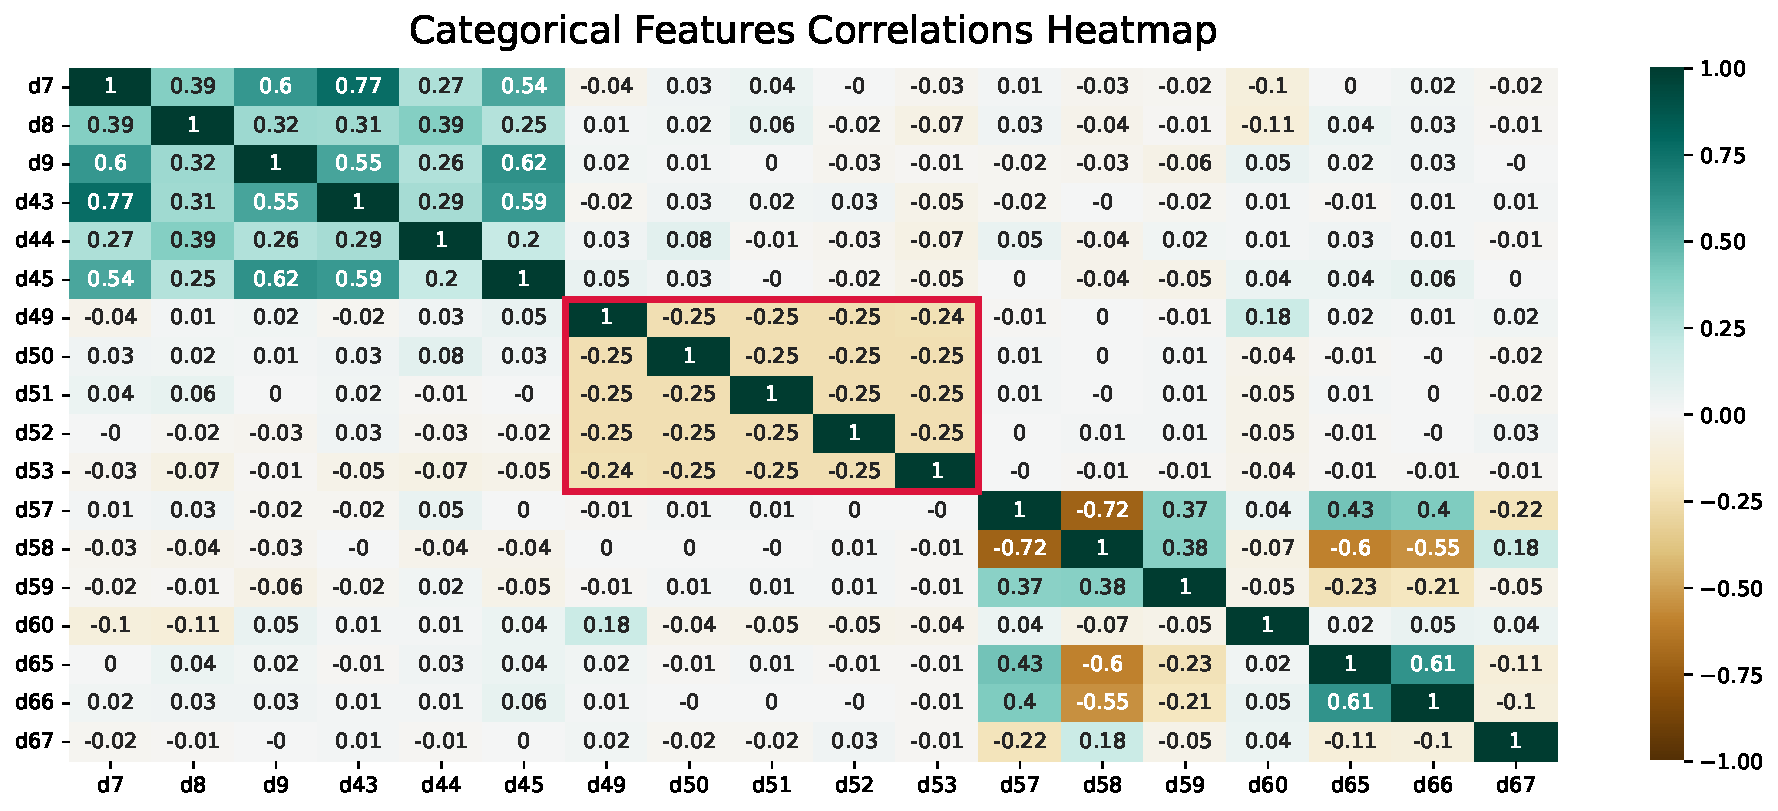
\includegraphics[width=0.85\textwidth]{collinearity} \\[0.5em]
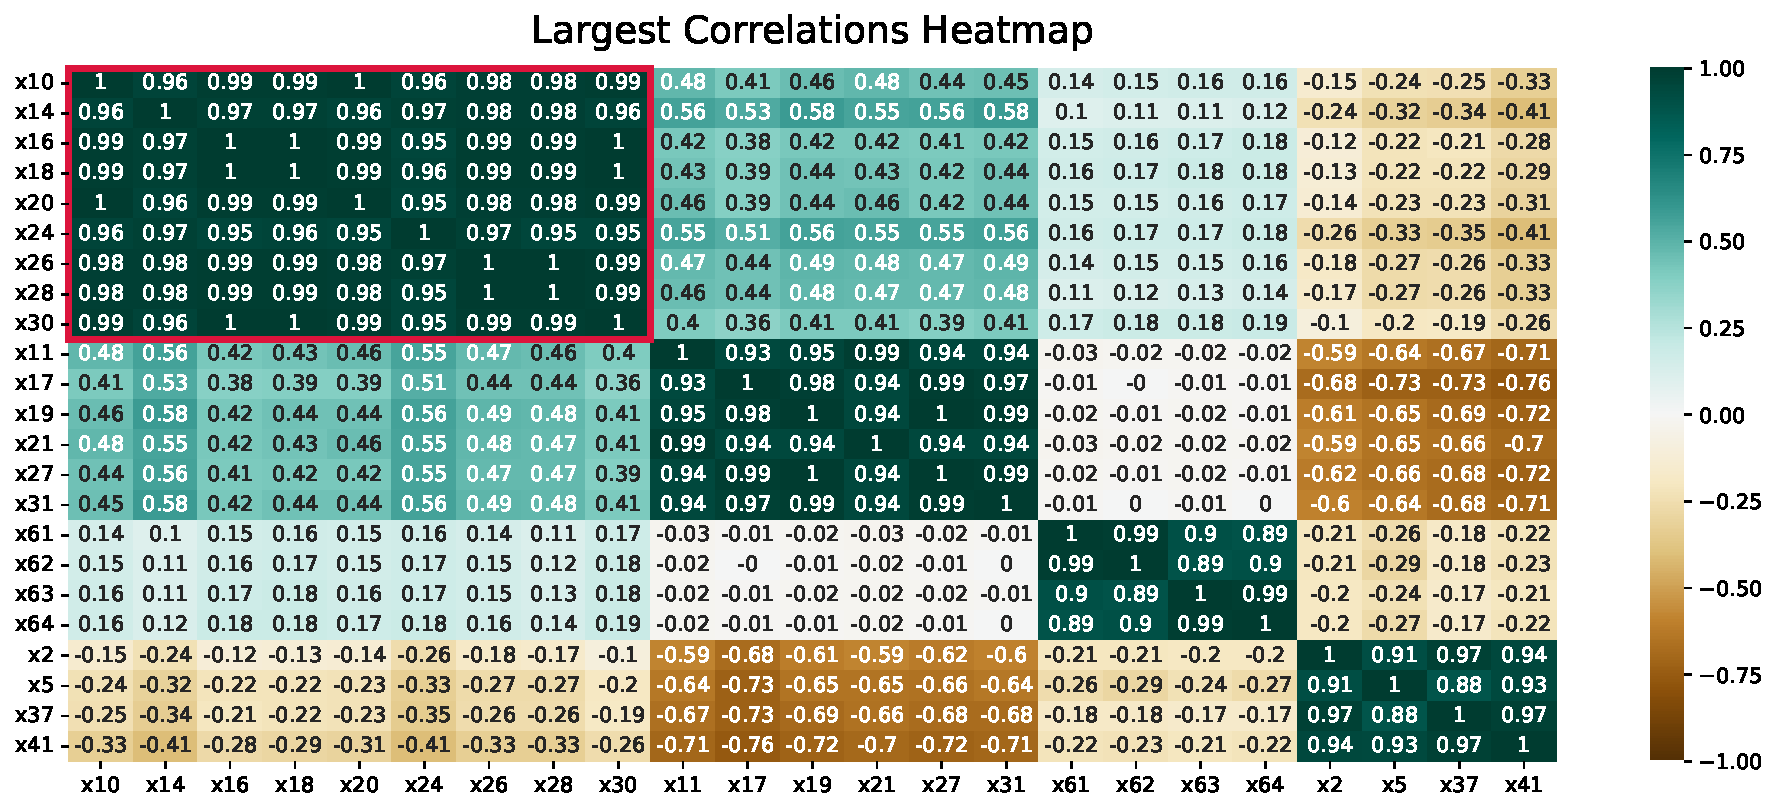
\includegraphics[width=0.85\textwidth]{corr_heatmap} \\[0.5em]
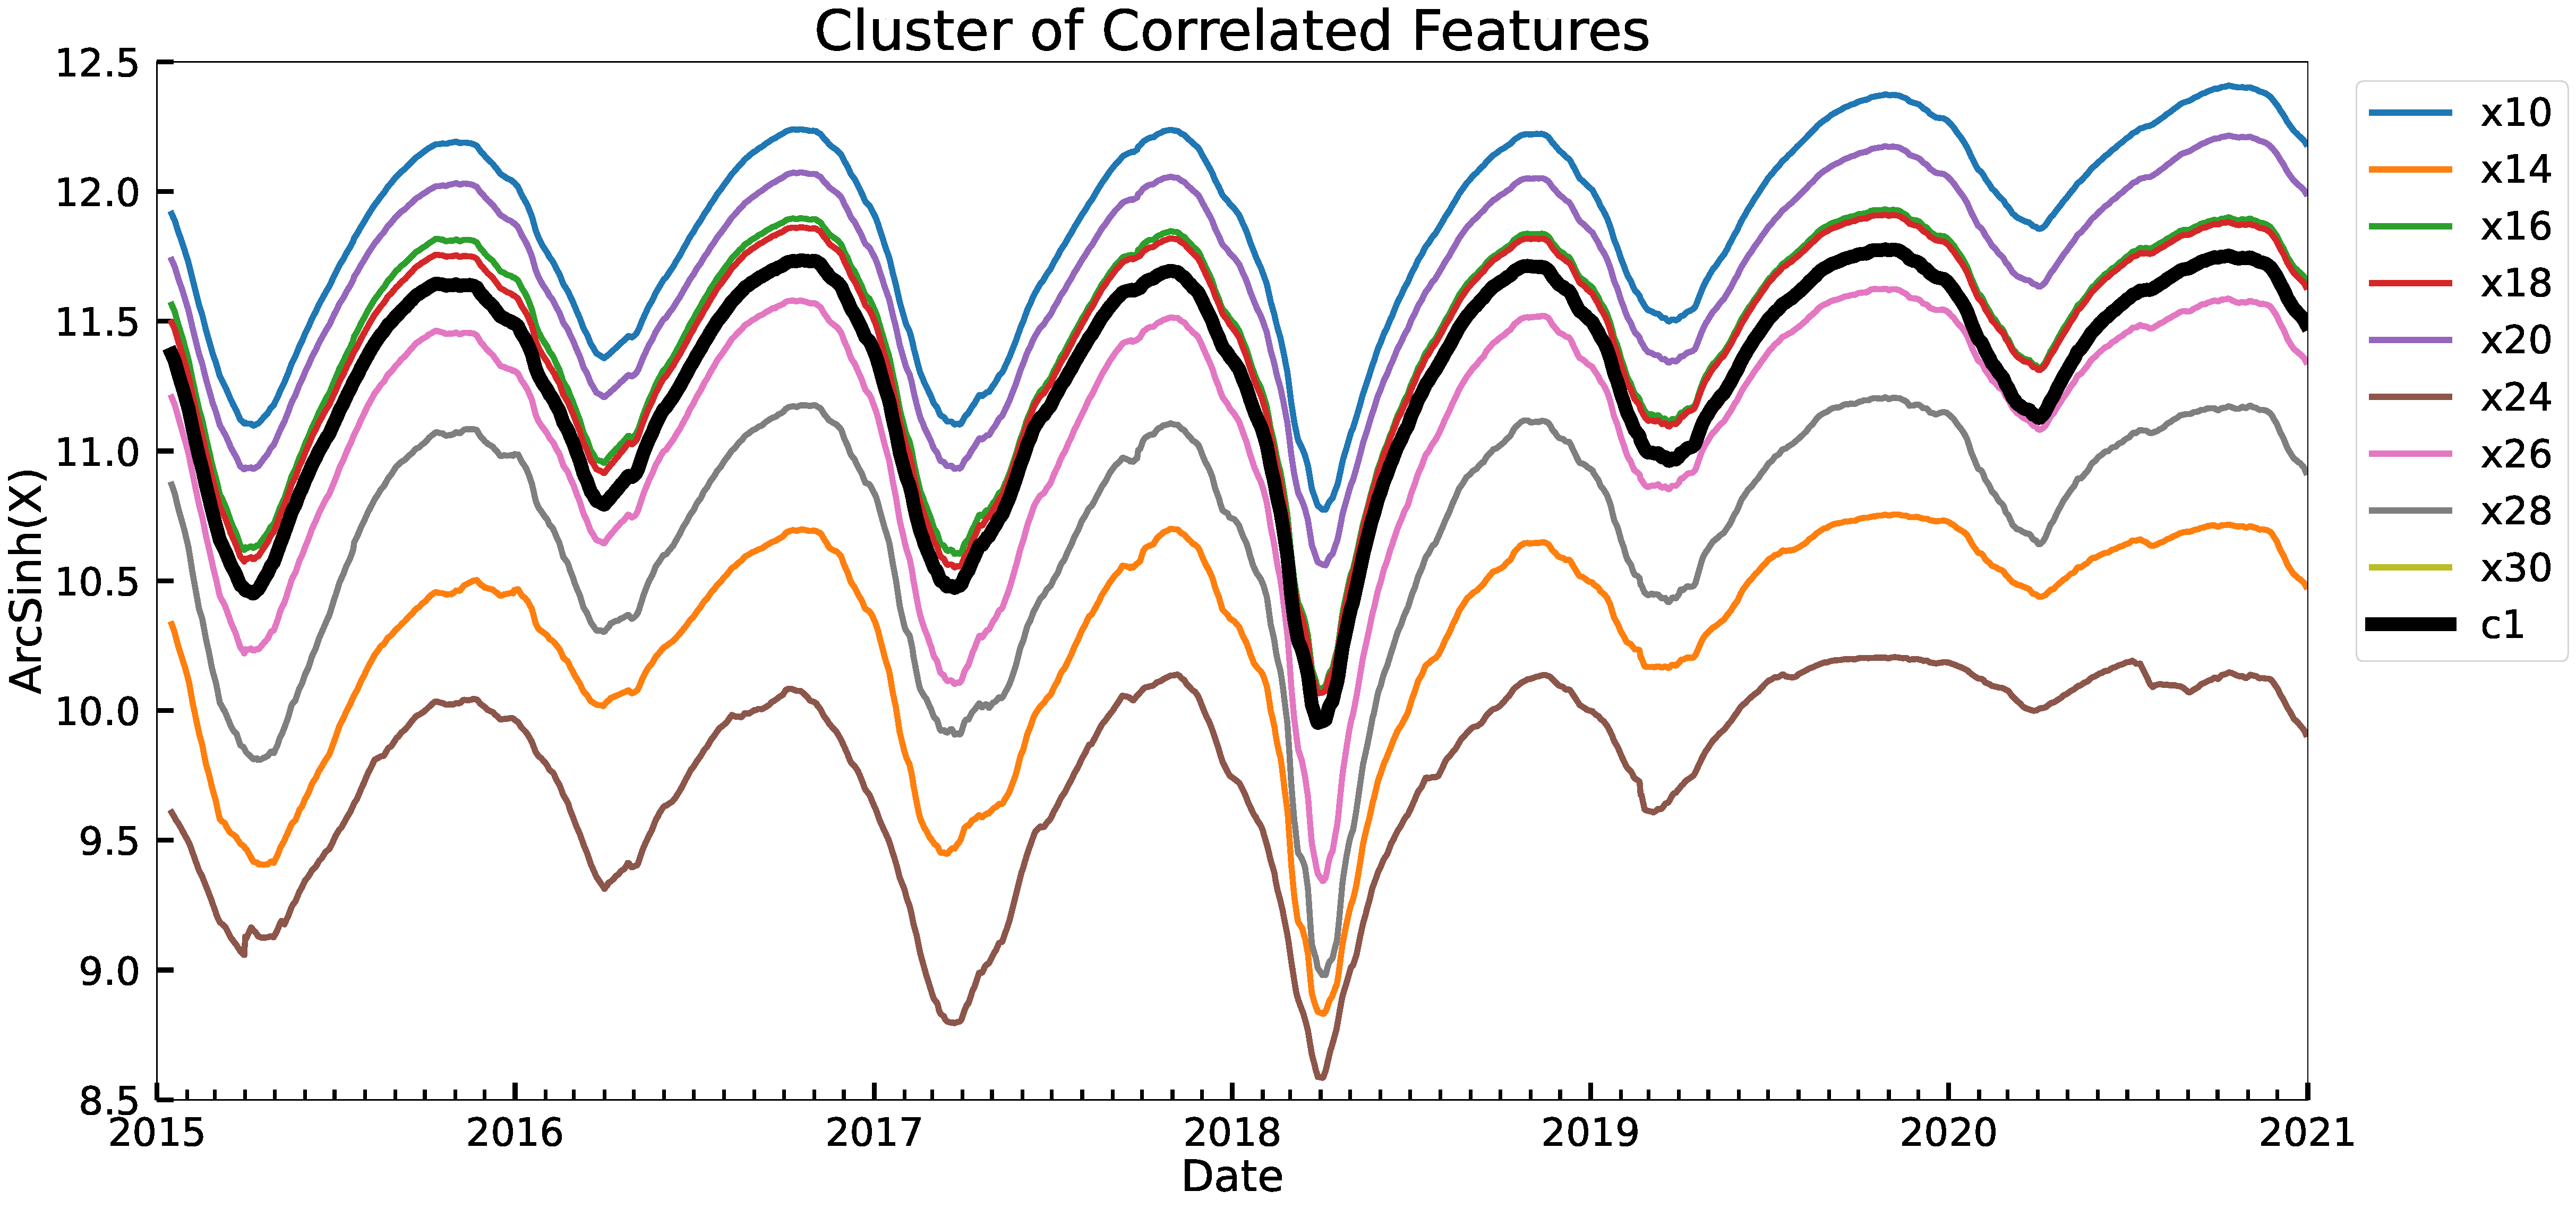
\includegraphics[width=0.85\textwidth]{cluster1} 
\caption{Correlation heatmap subset that highlights the identification of clustered variables based on Pearson correlation (top row) and time series of clustered features along with the representative median series that is used for model fits (bottom row).}
\label{fig:cluster}
\end{figure}

\begin{table}[ht]
\centering\small
\caption{Constituents of clustered features.}
\label{tab:clusters}
\begin{tabular}{cl}
\toprule
Cluster	&	\multicolumn{1}{c}{Constituent Features} \\ \midrule
c1	&	$x47$	,	$x48$	,	$x61$	,	$x62$	,	$x63$	,	$x64$	\\
c2	&	$x10$	,	$x14$	,	$x16$	,	$x18$	,	$x20$	,	$x24$	,	$x26$	,	$x28$	,	$x30$	\\
c3	&	$x70$	,	$x71$	,	$x73$	,	$x75$	,	$x81$	\\
c4	&	$x2$	,	$x5$	,	$x37$	,	$x41$		\\
c5	&	$x3$	,	$x38$	\\
c6	&	$x33$	,	$x90$	\\
c7	&	$x32$	,	$x79$	,	$x91$	\\
c8	&	$x11$	,	$x15$	,	$x17$	,	$x19$	,	$x21$	,	$x27$	,	$x29$	,	$x31$		\\
\bottomrule
\end{tabular}
\end{table}


\section{Model estimation and strategy formation}

\subsection{Strategy and benchmark weights}

The estimation methodologies attempt to forecast return values. Equation (\ref{eq:weights}) shows a logistic function that transforms the return forecast into a normalized weight for holding long or shorting the security:
\begin{align}
	w_t = \frac{2}{1+e^{-10\hat y_t}} - 1 \ ,
	\label{eq:weights}
\end{align}
where $\hat y_t$ is the return prediction and $w_t:\mathbb{R}\rightarrow[-1,1]$ is the security weight at time $t$. When $|\hat y_t|\rightarrow 0$ the signal is weak and the strategy is more conservative. However, when the prediction is large in absolute magnitude (strong signal) the security weight tilts rapidly towards 1 or -1 depending on the direction of the prediction.

I compare the proposed strategies with two simple benchmarks. The first is long the asset with $w_t=1$, i.e. simply buying the asset in the beginning and holding it. The second is a simplified momentum strategy, where equation (\ref{eq:weights}) transforms into a weight the 3-day rolling cumulative return.

\subsection{Estimation methodology}

I use two modeling processes, a custom stepwise regression built on linear estimations and the other on random forests. The former provides for economic interpretability and a simplified feature importance analysis, but it can be affected by collinearity. The latter can capture nonlinearities in the data generating process but it can be subject to overfitting.

The fundamental component of the stepwise algorithm is a rolling-window OLS regression. It includes time-varying exposures to the features and focuses on the most recent observations to derive the exposures for each period. The performance metric that is used to select the features is the Out-of-sample Adjusted R-squared (OAR), unlike the $p$-values that can result in overfitting. The out-of-sample setup implies that every rolling window is using information within the interval $[t-win-1, t-1]$ to make a prediction $\hat y_t$ at time $t$, where $win=300$ is the size of the time window. This size was chosen to capture the dynamics within one cycle across many feature time series that tend to have annual seasonality.

The feature selection logic is the following:
\begin{enumerate}
	\item Test every feature individually and keep only those that have OAR above a minimum threshold. This results in a dimensionality reduction before the stepwise selection begins.
	\item Start with the feature of maximum OAR from the previous stage and test every remaining feature with 2-variable regressions. The second feature will be the one that provides the largest OAR improvement relative to stage 1.
	\item Repeat the process in stage \#2 by adding features recursively until no further OAR improvement is feasible or the list of candidate features is exhausted.
\end{enumerate}

This process usually selects a parsimonious basket of features, because the required improvement in prediction for every stage is out-of-sample and not easy to achieve. In addition, the order that the features are selected implies a feature importance analysis by construction. The most important feature is selected first, the second feature selected is the next most important, and so on until the last selected feature has the least non-zero importance score.

The random forest estimation method is built similarly to the stepwise regression, where a different forest is trained within the same interval $[t-win-1, t-1]$ and the prediction $\hat y_t$ is made at time $t$. This approach intends to make the two methods consistent by embedding the assumption that only the most recent $win$ observations are valuable for prediction. Similarly to the stepwise regression, the method avoids imputed look-ahead biases and guarantees that security returns are predicted based on the information that is available until time $t-1$.

The performance evaluation process involves a dual lagging of variables to ensure that no look-ahead biases are artificially introduced. Intuitively, the models predict $\hat y_t$ given the information about the features until time $t-1$. This forecast is then converted to a strategy weight at time $t$, and profits are realized at time $t+1$. For instance, the sequence of prediction and realized profits for the linear model is the following:
\begin{enumerate}
	\item $b_{t-1}f_t = \hat y_t$, where $f_t$ the vector of features and $b_{t-1}$ their time-varying exposures.
	\item We buy or sell $w_t$ of the security at time $t$.
	\item The realized profit is $w_ty_{t+1}$ at time $t+1$.
\end{enumerate}

\begin{table}[ht]
\centering\small
\caption{Strategy performance evaluation.}
\label{tab:performance}
\begin{tabular}{ccccc}
\toprule
\multirow{2}{*}{Strategy}		&	\multicolumn{2}{c}{Full Sample} &	\multicolumn{2}{c}{Backtest} \\ %\midrule
 &	Sharpe Ratio & Max Drawdown &	Sharpe Ratio & Max Drawdown \\ \midrule
rOLS	&	1.01	&	-8.90		&	2.36	&	-1.64		\\
RF		&	0.99	&	-9.73		&	2.09	&	-1.47		\\
Mom		&	-0.17	&	-11.38	&	-0.40	&	-3.37		\\
Long	&	0.27	&	-11.98	&	1.75	&	-3.66		\\
\bottomrule
\end{tabular}
\end{table}


\subsection{Empirical results and backtesting}

The features selected by the stepwise regression are (in order of decreasing importance): $x40$, $d8$, $x85$, $d44$, $c5$, $d43$ and $x42$. The optimal model performance attained is $OAR=0.8$. Table \ref{tab:clusters} shows that cluster $c5$ combines the features $x3$ and $x38$.\footnote{A supplementary feature importance analysis using Shapley values on the random forest model could cross-validate the results from the stepwise regression.} Table \ref{tab:performance} and Figure \ref{fig:performance} summarize the empirical performance and PnL properties of each strategy, where rOLS represents the stepwise regression, RF the random forest, Mom the momentum strategy and Long is holding the asset.

Strategies rOLS and RF exhibit similar prediction capabilities and outperform the benchmarks. The outperformance stems from predicting correctly the direction of large jumps in the realized security returns and configuring the weights accordingly. Thus, they benefit both by buying and shorting the asset during those jumps. The drawdowns for the proposed strategies are smaller compared to the benchmark strategies.

\begin{figure}[htbp]
\centering
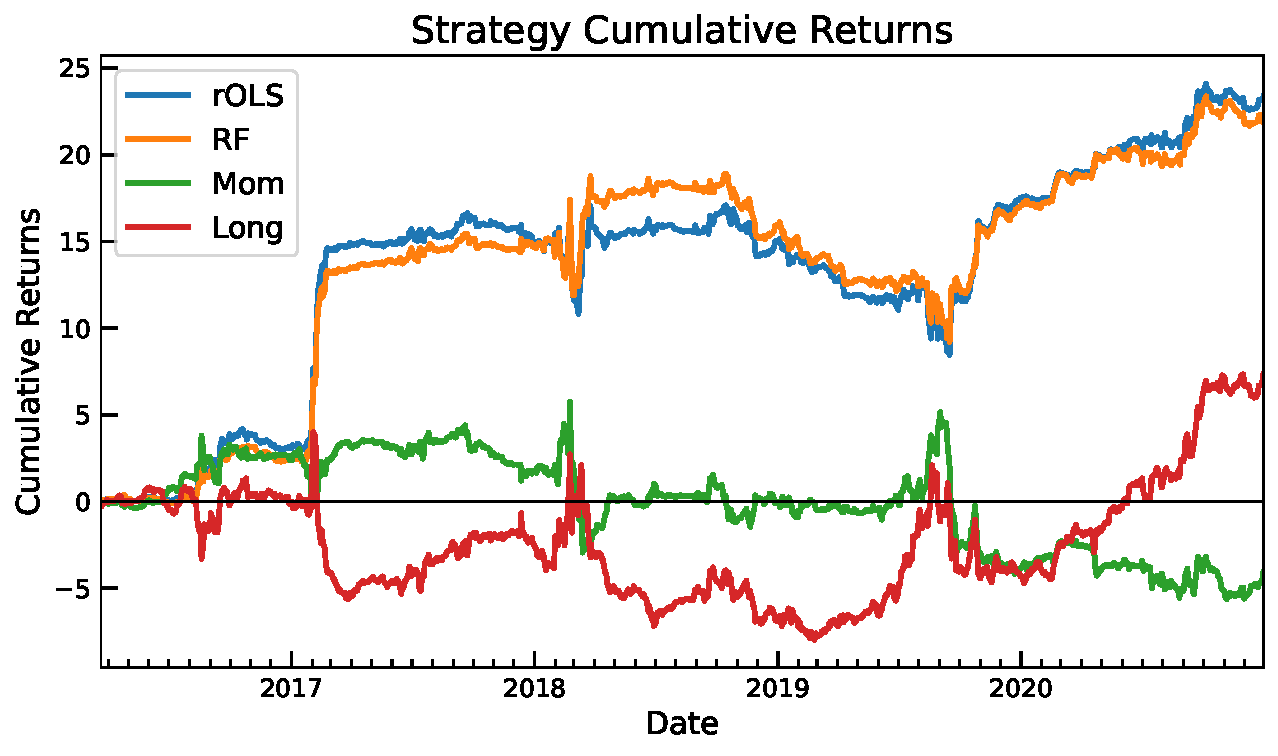
\includegraphics[width=0.45\textwidth]{cumret}
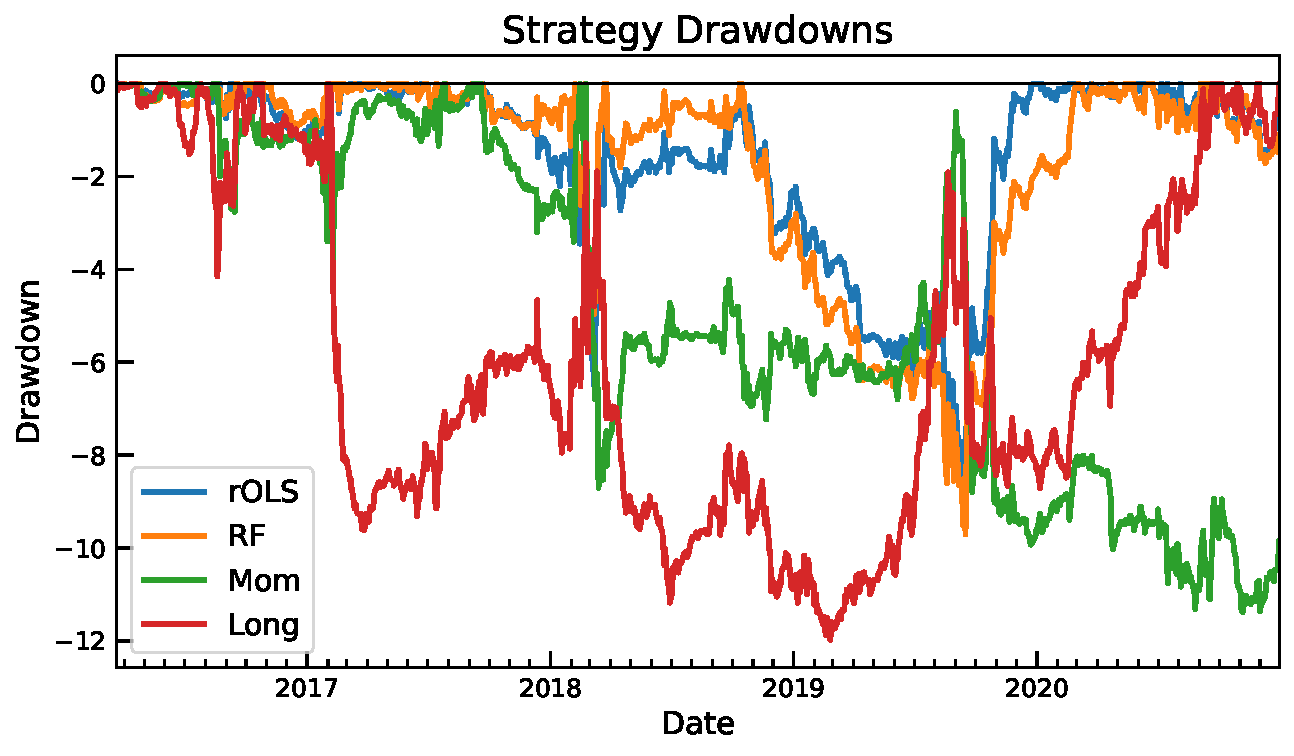
\includegraphics[width=0.45\textwidth]{drawdowns} \\
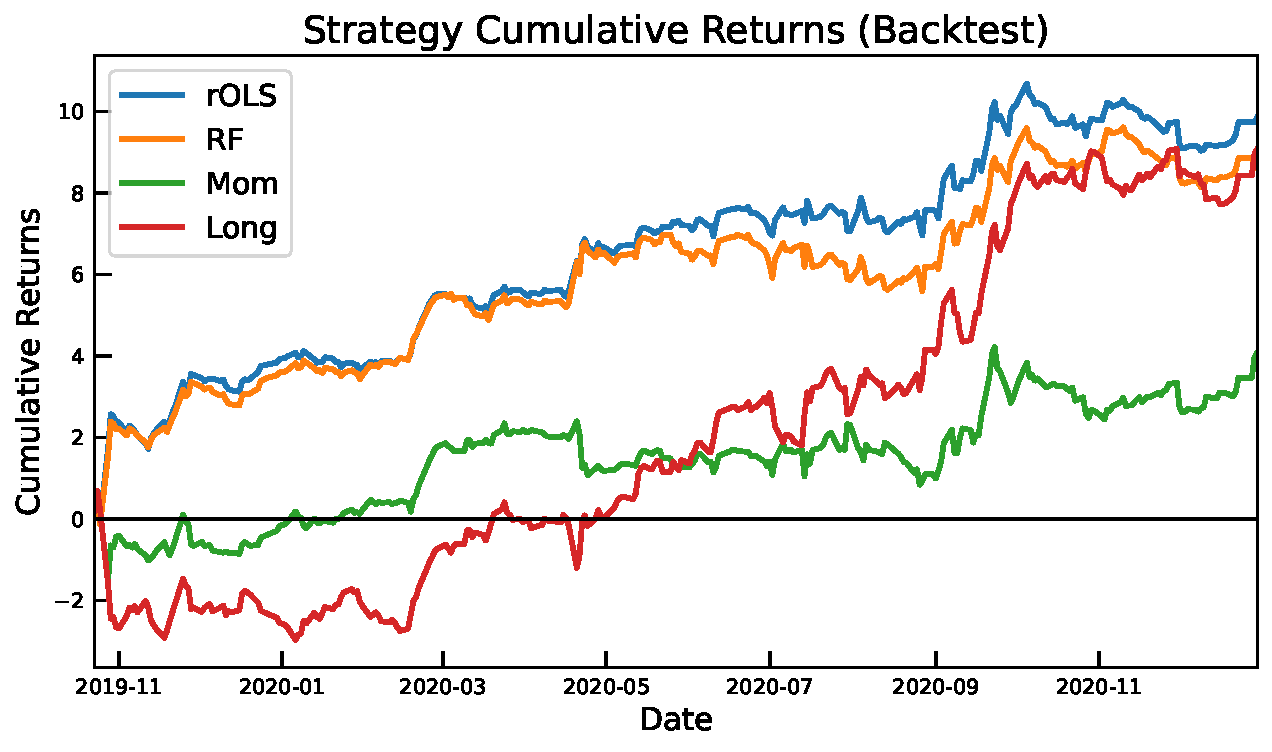
\includegraphics[width=0.45\textwidth]{cumret_backtest}
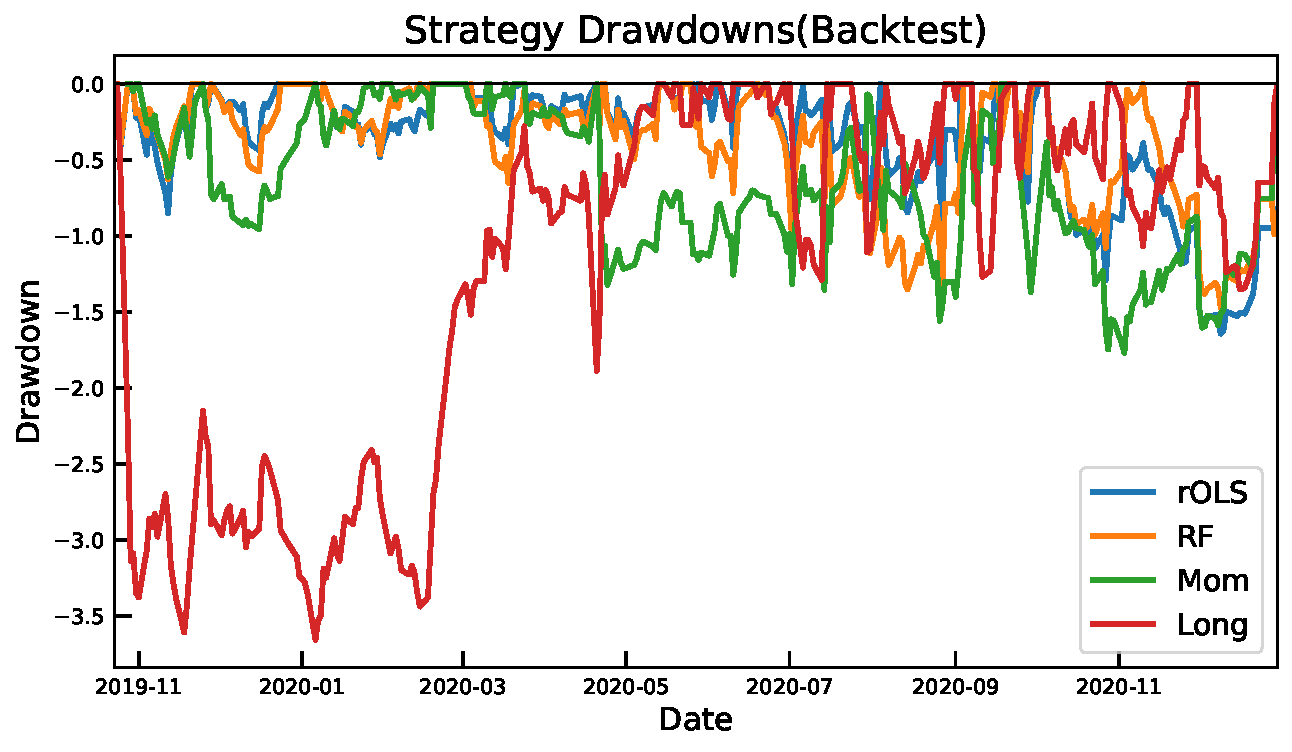
\includegraphics[width=0.45\textwidth]{drawdowns_backtest}
\caption{Strategy cumulative returns (left column row) and drawdowns (right column). The top row corresponds to the out-of-sample strategy performance across the full sample period and the bottom row to a backtest where the model is trained during the pre-Covid era and tested during the pandemic.}
\label{fig:performance}
\end{figure}

The analysis also includes a backtest to cross-validate the model performance for more than one periods ahead. The backtest is configured such that the state of the economy is different between the training and testing sets. In particular, the models are estimated before the Covid-19 era and then their performance is tested during the pandemic. Once again, the strategies rOLS and RF exhibit similar prediction capabilities and outperform the benchmarks.



\end{document}